\documentclass[journal]{IEEEtran}
\usepackage[a5paper, margin=10mm, onecolumn]{geometry}
\usepackage{lmodern}

\setlength{\headheight}{1cm}
\setlength{\headsep}{0mm}

\usepackage{gvv-book}
\usepackage{gvv}
\usepackage{cite}
\usepackage{amsmath,amssymb,amsfonts,amsthm}
\usepackage{graphicx}
\graphicspath{{./figs/}}
\usepackage{xcolor}
\usepackage{txfonts}
\usepackage{enumitem}
\usepackage{mathtools}
\usepackage{hyperref}
\usepackage{tikz}
\usepackage{tkz-euclide}

\begin{document}

\bibliographystyle{IEEEtran}
\vspace{3cm}

\title{1.9.25}
\author{EE25BTECH11036 - M Chanakya Srinivas}
\maketitle

\renewcommand{\thetable}{\theenumi}
\setlength{\intextsep}{10pt}
\renewcommand\theequation{\arabic{equation}}

\textbf{Question 1.9.25:}  
If the point $P(x,y)$ is equidistant from $A(a+b, b-a)$ and $B(a-b, a+b)$,  
prove that $bx = ay$.

\bigskip
\textbf{Solution:}

\medskip
\textbf{1. Given Data}  

Define
\begin{align}
\vec{z} &= \myvec{a \\ b}. \label{eq:z-def}
\end{align}

Then
\begin{align}
\vec{A} &= \myvec{1 & 1 \\ -1 & 1}\vec{z}, \label{eq:A-def} \\
\vec{B} &= \myvec{1 & -1 \\ 1 & 1}\vec{z}, \label{eq:B-def} \\
\vec{P} &= \myvec{x \\ y}. \label{eq:P-def}
\end{align}

Notice that
\begin{align}
\myvec{1 & -1 \\ 1 & 1} 
= \myvec{1 & 1 \\ -1 & 1}^T 
\quad \Rightarrow \quad 
\vec{B} = \vec{A}^T \vec{z}. \label{eq:B-ATz}
\end{align}

\medskip
\textbf{2. Equidistant Condition}
\begin{align}
\norm{\vec{P}-\vec{A}}^2 &= \norm{\vec{P}-\vec{B}}^2, \\
(\vec{P}-\vec{A})^T(\vec{P}-\vec{A}) &= (\vec{P}-\vec{A}^T)^T(\vec{P}-\vec{A}^T).
\end{align}

\medskip
\textbf{3. Simplification using $B=A^T$}
\begin{align}
2(\vec{A}^T - \vec{A})^T \vec{P} &= \vec{A}^{T}\vec{A}^{T} - \vec{A}^T\vec{A}.
\end{align}

But since $\vec{A}^T\vec{A}$ is symmetric,  
\begin{align}
\vec{A}^{T}\vec{A}^{T} - \vec{A}^T\vec{A} = 0.
\end{align}

Hence
\begin{align}
(\vec{A}^T - \vec{A})^T \vec{P} = 0.
\end{align}

\medskip
\textbf{4. Final Result}
Expanding,
\begin{align}
(\vec{B}-\vec{A})^T\vec{P} 
&= \Bigg(\myvec{0 & -2 \\ 2 & 0}\vec{z}\Bigg)^T \vec{P}, \\
&= -2bx + 2ay = 0, \\
\Rightarrow \quad bx &= ay.
\end{align}

\begin{figure}[H]
    \centering
    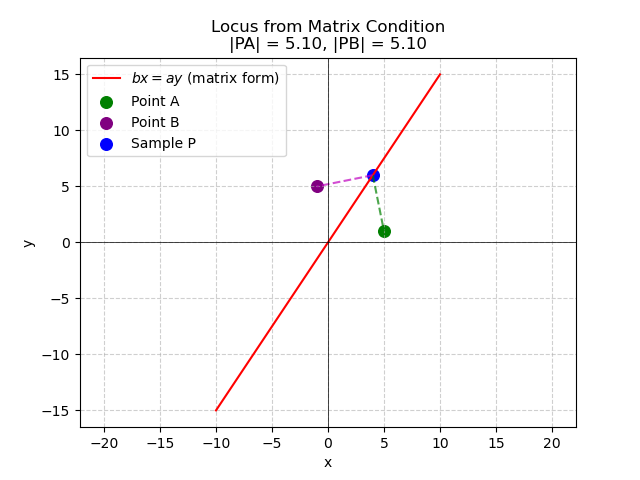
\includegraphics[width=0.9\linewidth]{figs/Fig1.png}
    \caption{}
\end{figure}

\begin{figure}[H]
    \centering
    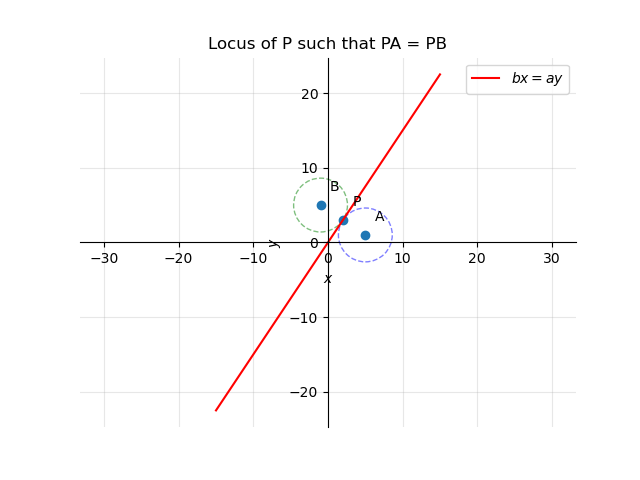
\includegraphics[width=0.9\linewidth]{figs/fig2.png}
    \caption{}
\end{figure}

\end{document}
